\documentclass{article}

\usepackage{graphicx}
\usepackage[margin=1in]{geometry}

\DeclareGraphicsExtensions{.png}

\begin{document}

\begin{center}

    \huge{\textbf{WhiteBoard}}

    \huge{\textit{An Efficient and Intuitive Learning Management System}}

    \huge{Project Proposal}

    \vspace{10 pt}

    \large{
        \begin{tabular}{cccc}
            Noah Christiano&Joel Kottas&Shir Maimon&Jacob Roschen\\
        \end{tabular}
    }

\end{center}

\vspace{10 pt}

\section{Background}

A Learning Management System(LMS) is an interface between students, professors,
and school administration. One of the most popular LMSes, especially at
colleges and universities, is Blackboard\cite{Blackboard}.  Blackboard,
however, like other LMSes, is extremely slow and has unnecessary features that
are often left unused. For example, Blackboard's personalize page features are
rarely used, and students avoid the discussion boards. These LMSes designs
also often make them difficult to navigate. For example, Blackboard has two
sets of navigation tabs, and it is not obvious what the difference between them
is. These problems add up to create an interface that is slow and difficult to
use, even though there is no need for it to be that way. Students today would
rather get what they need quickly than have hundreds of features that they
rarely, if ever, use. Other LMSes exist too, such as Moodle\cite{Moodle},
Veracross\cite{Veracross}, and Canvas\cite{Canvas}, but they have their own
problems, and none of them are open-source or as lightweight as we want.

\section{Objective}

WhiteBoard will focus on having an efficient, intuitive interface, and it will
have features of excellent quality rather than a large quantity of features. It
is open-source, allowing it to be customized and used as desired, although it
focuses on the University of Rochester. Most importantly, WhiteBoard will have
a unified user experience. It shouldn't take a student who is majoring in
computer science three days to find where the grades are posted, and even then
to be confused about what their grade is, and it should be easy to navigate to
the University of Rochester website. WhiteBoard's design will make such
navigation a pleasure.

\section{Features}

Specifically, WhiteBoard will have the following features:
\begin{itemize}
    \item Lightning-quick load times
    \item A secure and painless login system
    \item Course system, with registration and grades for students
    \item Schudule and calendar
    \item Convenient communication between administrators, professors, and
        students, both for general communication and announcements
    \item Open source
\end{itemize}

\section{Current Assets}

Our team's combined experience covers PHP and Javascript very well, the LAMP
stack and all its associated programming languages, and even configuring a
Linux server for web hosting. Everyone on the team understands design, and how
to learn from both the successes and the mistakes of systems like Blackboard.
As students, we have constant access to Blackboard, and we have the expertise
to dive into the site to see what code works well and what code doesn't. We are
also constantly learning, and our ability in areas relating to this project
will only increase.

We are also using several libraries to assist in creating WhiteBoard. We are
using jQuery, a javascript library, and code from the open source PHP-Login
project, so that we have a secure but simple to use system. There are also many
other libraries for Javascript and PHP available should we find them useful.

\section{Budget}

A large budget shouldn't be necessary. WhiteBoard requires server space on
which it can be hosted, but we are planning to get server space on the computer
science servers to save money. If we can't get server space there, then we
shouldn't need to spend more than \$10 per month on hosting.

\section{Schedule and Plan}

\vspace{10 pt}

\begin{tabular}{ll}
    Expected Date Done&Feature(s)\\
    10/23/14&Development environment and datbase structure\\
    10/25/14&Login system and general layout\\
    11/1/14&Courses and grades\\
    11/8/14&Announcements and communication\\
    11/15/14&Schedule/calendar\\
    11/29/14&Presentation\\
\end{tabular}

\subsection{Development Environment}

We are collaborating over GitHub, which combines version control, file sharing,
and the ability to edit files online into one service.

We will rent a dedicated server from Online hosting. This Ubuntu server hosts a
LAMP stack which is the foundation for the website. The web server hosts two
copies of the website, one with a functioning version of the site and another
with a test version of the site. This allows us to push changes to the server
via GitHub and test our code in real time. The database will use MySQL and the
SQL programming language. Our database structure will be similar to the open
source moodle project's. However, ours will be greatly simplified in order to
promote efficiency.

\subsection{Database Structure}

We have thoroughly planned the database for the entire system. Fundamentally,
the database dictates how the PHP code is organized and implemented. A diagram
of the database structure follows.

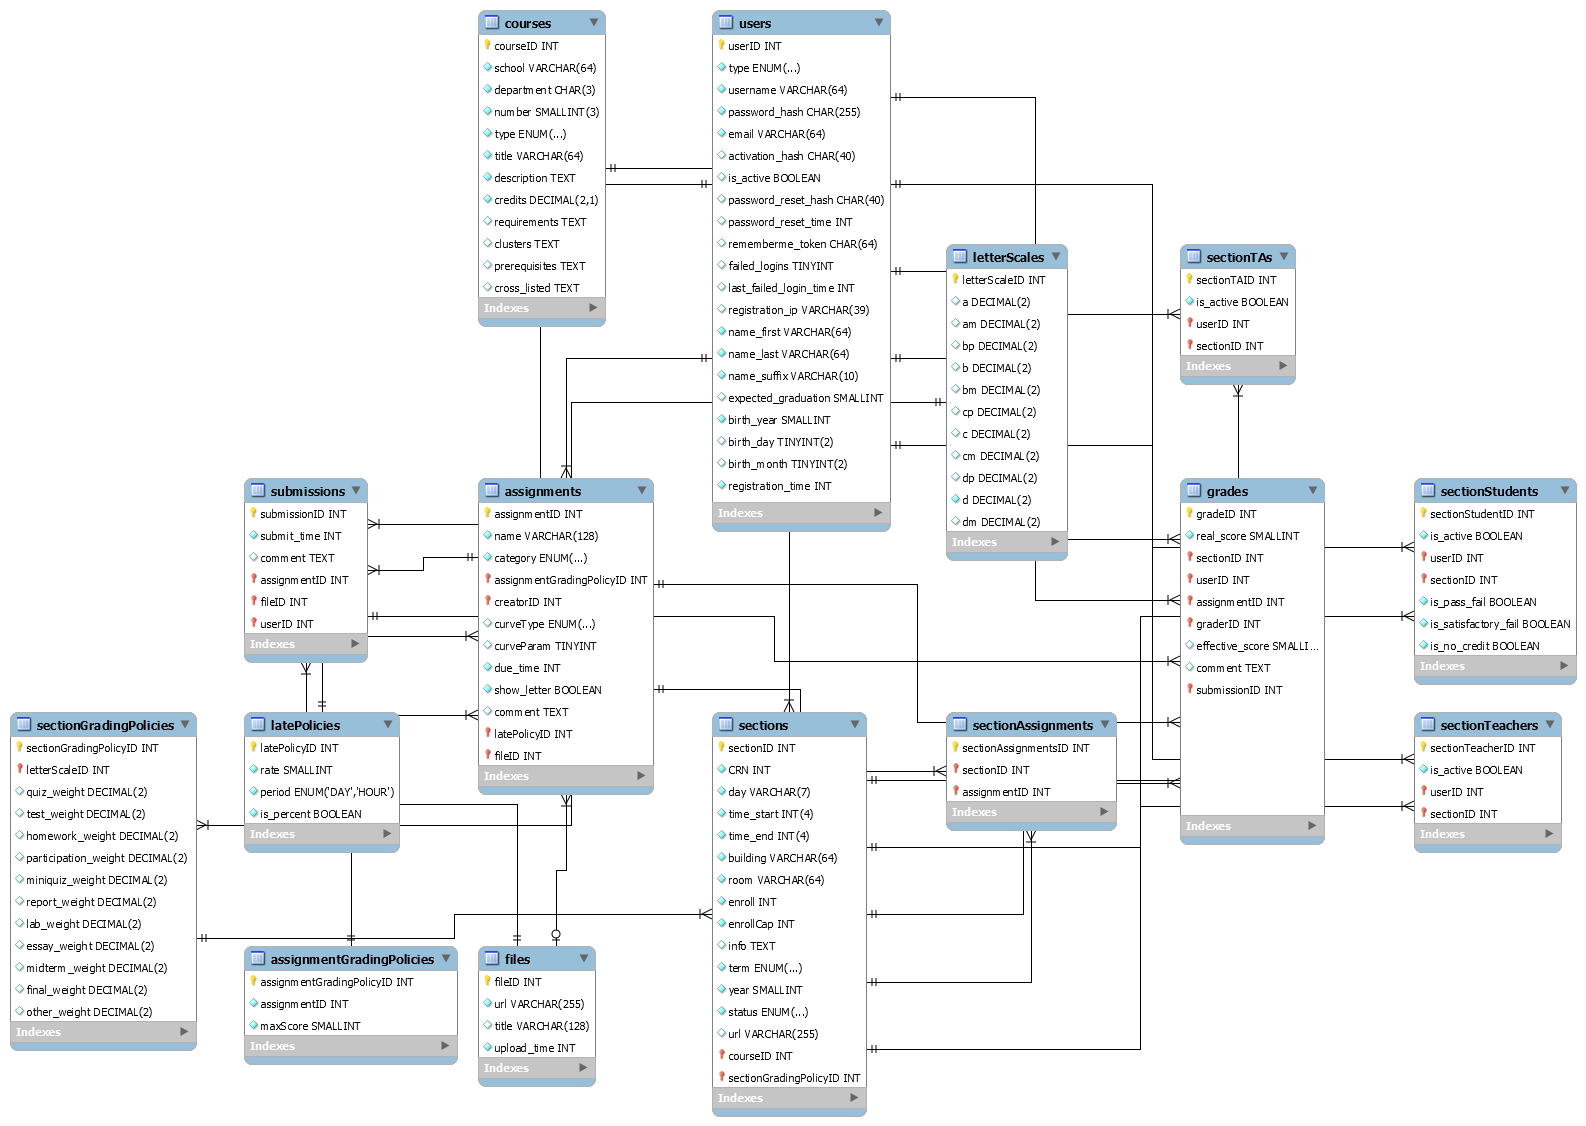
\includegraphics[width=6.5 in]{db}

\subsection{Login System}

With the open-source library we're using, the PHP-Login project, most of the
login system is complete. Some adjustments for our front-end and our database
structure may be necessary, but they should be fairly small.

\subsection{General Layout}

The general layout of the page is straightforward: there is a header, sidebar,
and the main content area. The goal of this project is not to make anything too
fancy, and keeping the user interface simple like this is one of the main ways
we accomplish this goal.

% \includegraphics[width=6.5 in]{example_page}

\subsection{Courses}

TEXT

\subsection{Grades}

TEXT

\subsection{Announcements}

TEXT

\subsection{Communication}

TEXT

\subsection{Schedule / Calendar}

TEXT

\subsection{Presentation}

TEXT

\bibliography{refs}{} \bibliographystyle{plain}

\end{document}
